% 1998 上海文科第20题解题辅助示意：不是原卷图形；坐标与割线仅作示例，不按比例。
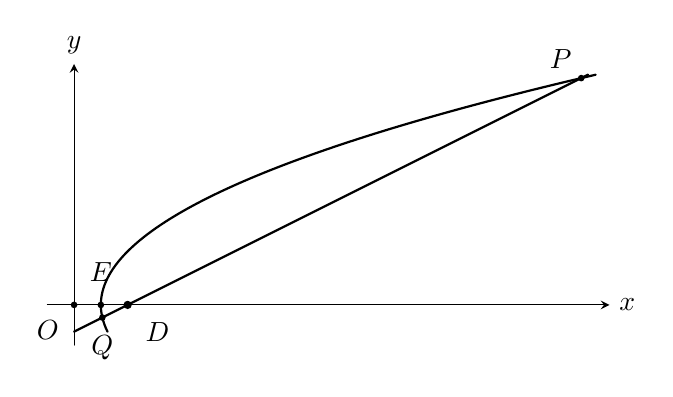
\begin{tikzpicture}[x=0.34cm,y=0.34cm,>=stealth,line cap=round,line join=round]
  \draw[->] (-1,0)--(20,0) node[right] {$x$};
  \draw[->] (0,-1.5)--(0,9) node[above] {$y$};
  \draw[thick,domain=-1:8.6,samples=120] plot ({1+\x*\x/4},{\x});
  % 示出一条过焦点D的示意割线（斜率 1/2，非答案构形）；不按比例。
  \draw[thick,domain=-1:8.6,variable=\y] plot ({2+2*\y},{\y});
  \coordinate (P) at ({2+2*(4+2*sqrt(5))},{4+2*sqrt(5)});
  \coordinate (Q) at ({2+2*(4-2*sqrt(5))},{4-2*sqrt(5)});
  \fill (0,0) circle (1.2pt) node[below left=2pt] {$O$};
  \fill (1,0) circle (1.2pt) node[above=5pt] {$E$};
  \fill (2,0) circle (1.5pt) node[below right=3pt] {$D$};
  \fill (P) circle (1.2pt) node[above left] {$P$};
  \fill (Q) circle (1.2pt) node[below=3pt] {$Q$};
  \end{tikzpicture}
